% mnras_template.tex 
%
% LaTeX template for creating an MNRAS paper
%
% v3.0 released 14 May 2015
% (version numbers match those of mnras.cls)
%
% Copyright (C) Royal Astronomical Society 2015
% Authors:
% Keith T. Smith (Royal Astronomical Society)

% Change log
%
% v3.0 May 2015
%    Renamed to match the new package name
%    Version number matches mnras.cls
%    A few minor tweaks to wording
% v1.0 September 2013
%    Beta testing only - never publicly released
%    First version: a simple (ish) template for creating an MNRAS paper

%%%%%%%%%%%%%%%%%%%%%%%%%%%%%%%%%%%%%%%%%%%%%%%%%%
% Basic setup. Most papers should leave these options alone.
\documentclass[fleqn,usenatbib]{mnras}

% MNRAS is set in Times font. If you don't have this installed (most LaTeX
% installations will be fine) or prefer the old Computer Modern fonts, comment
% out the following line
\usepackage{newtxtext,newtxmath}
% Depending on your LaTeX fonts installation, you might get better results with one of these:
%\usepackage{mathptmx}
%\usepackage{txfonts}

% Use vector fonts, so it zooms properly in on-screen viewing software
% Don't change these lines unless you know what you are doing
\usepackage[T1]{fontenc}
\usepackage{subfig} %for figure subplot
\usepackage{graphicx}
\usepackage[flushleft]{threeparttable}
\usepackage{xspace}

%%%%%%%%%%%%%%%%%%%%%%%%%%%%%%%%%%%%%%%%%%%%%%%%%%%%%%%%%%%%%%%%%%%
% my commands
\newcommand{\lcdm}{$\Lambda$CDM}
\newcommand{\hst}{{\it HST}}
\newcommand{\hc}{$H_0$}
\newcommand{\efr}{$R_{\mathrm{eff}}$}
\newcommand{\galfit}{{\sc Galfit}}
\newcommand{\mbh}{$\mathcal M_{\rm BH}$}
\newcommand{\lhost}{$L_{\rm host}$}
\newcommand{\mr}{$Mag_{\rm ~R}$}
\newcommand{\halpha}{H$_{\alpha}$}
\newcommand{\Hb}{H$_{\beta}$}
\newcommand{\sersic}{S\'ersic}
\newcommand{\lenstronomy}{{\sc Lenstronomy}}
\newcommand{\reff}{{$R_{\mathrm{eff}}$}}
\newcommand{\kmsMpc}{km~s$^{\rm -1}$~Mpc$^{\rm -1}$}
\newcommand{\kms}{\ifmmode{\,\rm{km}\, \rm{s}^{-1}}\else{$\,$km$\,$s$^{-1}$}\fi}
\newcommand{\sigstar}{{$\sigma_*$}}
\newcommand{\mstar}{{$M_*$}}
\newcommand{\Mgii}{Mg$_{\rm II}$}
\newcommand{\Civ}{C$_{\rm IV}$}
%\newcommand{\farcs}{\mbox{\ensuremath{.\!\!^{\prime\prime}}}}% fractional arcsecond symbol: 0.''0
\newcommand{\sam}{\texttt{SAM}}
\newcommand{\mbii}{\texttt{MBII}}
%%%%%%%%%%%%%%%%%%%%%%%%%%%%%%%%%%%%%%%%%%%%%%%%%%%%%%%%%%%%%%%%%%%
\newcommand{\ding}[1]{\textcolor{red}{[{\bf Xuheng}: #1]}}
\newcommand{\todo}[1]{\textcolor{red}{[{\bf Todo}: #1]}}  
\newcommand{\red}[1]{{ \textcolor{red}{#1}}}
\newcommand{\blue}[1]{{ \textcolor{blue}{#1}}}
\newcommand{\pink}[1]{{ \textcolor{magenta}{#1}}}

% Allow "Thomas van Noord" and "Simon de Laguarde" and alike to be sorted by "N" and "L" etc. in the bibliography.
% Write the name in the bibliography as "\VAN{Noord}{Van}{van} Noord, Thomas"
\DeclareRobustCommand{\VAN}[3]{#2}
\let\VANthebibliography\thebibliography
\def\thebibliography{\DeclareRobustCommand{\VAN}[3]{##3}\VANthebibliography}


%%%%% AUTHORS - PLACE YOUR OWN PACKAGES HERE %%%%%

% Only include extra packages if you really need them. Common packages are:
\usepackage{graphicx}	% Including figure files
\usepackage{amsmath}	% Advanced maths commands
\usepackage{amssymb}	% Extra maths symbols

%%%%%%%%%%%%%%%%%%%%%%%%%%%%%%%%%%%%%%%%%%%%%%%%%%

%%%%% AUTHORS - PLACE YOUR OWN COMMANDS HERE %%%%%

% Please keep new commands to a minimum, and use \newcommand not \def to avoid
% overwriting existing commands. Example:
%\newcommand{\pcm}{\,cm$^{-2}$}	% per cm-squared

%%%%%%%%%%%%%%%%%%%%%%%%%%%%%%%%%%%%%%%%%%%%%%%%%%

%%%%%%%%%%%%%%%%%%% TITLE PAGE %%%%%%%%%%%%%%%%%%%

% Title of the paper, and the short title which is used in the headers.
% Keep the title short and informative.
\title[Mass relations by lensed AGN hosts]{The Mass Relations between Supermassive Black Holes and Their Host Galaxies using Eight Strongly Lensed AGN Systems.}

% The list of authors, and the short list which is used in the headers.
% If you need two or more lines of authors, add an extra line using \newauthor
\author[X. Ding et al.]{
Xuheng Ding$^{1}$\thanks{E-mail: dxh@astro.ucla.edu},
Tommaso Treu$^{1}$,
Simon Birrer$^{2}$,
Dominique Sluse$^{3}$,\newauthor
Chris Fassnacht$^{4}$,
Matthew W. Auger$^{5}$,
Kenneth C. Wong$^{6}$,
Sherry H. Suyu$^{7,8,9}$,\newauthor
Takahiro Morshita$^{10}$,
and et al.
\\
% List of institutions
$^{1}$Department of Physics and Astronomy, University of California, Los Angeles, CA, 90095-1547, USA\\
$^{2}$Kavli Institute for Particle Astrophysics and Cosmology and Department of Physics, Stanford University, Stanford, CA 94305, USA\\
$^{3}$STAR Institute, Quartier Agora - All\'ee du six Ao\^ut, 19c B-4000 Li\`ege, Belgium\\
$^{4}$Department of Physics, University of California, Davis, CA 95616, USA\\
$^{5}$Institute of Astronomy, University of Cambridge, Madingley Road, Cambridge CB3 0HA, UK\\
$^{6}$Kavli IPMU (WPI), UTIAS, The University of Tokyo, Kashiwa, Chiba 277-8583, Japan\\
$^{7}$Max-Planck-Institut f{\"u}r Astrophysik, Karl-Schwarzschild-Str.~1, 85748 Garching, Germany\\
$^{8}$Physik-Department, Technische Universit\"at M\"unchen, James-Franck-Stra\ss{}e~1, 85748 Garching, Germany\\
$^{9}$Academia Sinica Institute of Astronomy and Astrophysics (ASIAA), 11F of ASMAB, No.1, Section 4, Roosevelt Road, Taipei 10617, Taiwan\\
$^{10}$Space Telescope Science Institute, 3700 San Martin Drive, Baltimore, MD 21218, USA
}

% These dates will be filled out by the publisher
\date{Accepted XXX. Received YYY; in original form ZZZ}

% Enter the current year, for the copyright statements etc.
\pubyear{2020}

% Don't change these lines
\begin{document}
\label{firstpage}
\pagerange{\pageref{firstpage}--\pageref{lastpage}}
\maketitle

% Abstract of the paper
\begin{abstract}
\todo{Needs to be rewritten.}
Strong lensed active galactic nuclei (AGN) has been considered as a unique tool to exam the correlations between the mass of the supermassive Black Hole and its host galaxies. In this work, we have adopted eight strongly lensed system from our collaboration. The deep {\it Hubble Space Telescope}(\hst) data and adopt the \lenstronomy\ to reconstruct the image of the source. Using the reconstructed brightness of the host galaxy, we infer the host galaxy stellar mass based on the assumed stellar population. 
The \mbh\ are estimated using the board emission line. We compare our inference to the ones in the literature and find a consistent result. The consistent scaling resolutions derived from our sample confirm the evolution conclusion and confirm the the power of using strong lensed AGNs. The number of the detection of the lensed AGNs are supposed to increase rapidly leave this topic with a bright future...
\end{abstract}

% Select between one and six entries from the list of approved keywords.
% Don't make up new ones.
\begin{keywords}
galaxies: evolution -- galaxies: active -- gravitational lensing: strong
\end{keywords}

%%%%%%%%%%%%%%%%%%%%%%%%%%%%%%%%%%%%%%%%%%%%%%%%%%

%%%%%%%%%%%%%%%%% BODY OF PAPER %%%%%%%%%%%%%%%%%%
\section{Introduction}
The tight correlations between the masses (\mbh) of supermassive black holes (BHs) and their host galaxies properties including stellar mass (\mstar), stellar velocity dispersion ($\sigma_*$) and luminosity (\lhost), known as scaling relations, are usually considered as a result of their co-evolution ~\citep[e.g.,][]{Mag++98, F+M00, Geb++01b, M+H03, Gul++09,Beifi2012, H+R04, Gra++2011}, whose origin is till unclear so far. In theory, cosmological simulations of structure formation are able to reproduce the local tight relation based on physical mechanism by invoking active galactic nucleus (AGN) feedback as the physical connection~\citep{Springel2005, Hopkins2008, Matteo2008, DeG++15} or having them share a common gas supply~\citep{Cen2015, Menci2016}. On the other hand, without any physical coupling, the pure statistical convergence by galaxy mergers alone could also reproduce the observed correlations at local universe~\citep{Peng2007, Jahnke2011, Hirschmann2010}. 

It is crucial to extend the correlation studies to higher redshift to study them as a function of redshift, determining how and when they emerge and evolve over cosmic time~\citep[e.g.,][]{TMB04,Sal++06,Woo++06, Jah++09,SS13,Sun2015, Park15}. Recently, based on a sample of 32 X-ray-selected type-1 AGNs in deep survey fields, \citet{Ding2020a} (hereafter, D20) measured the scaling relations at redshift range up to $1.2<z<1.7$ using \hst\ imaging with WFC3. Combining with the published samples in both local and intermediate redshift range, they confirm the evolution scenario that the growth of BHs evolution predates than the bulge component of the host galaxy. In a following up work, \citep{Ding2020b} compared their measurements to the predictions by the numerical simulations including the hydrodynamic simulation MassiveBlackII~\citep{Khandai2015} and a semi-analytic model~\citep{Menci2014}. The tightness of the observed scaling relations at high-$z$ supports the hypothesis that AGN feedback as a promising driver for the scaling correlations. Apparently, a larger sample at the higher redshift range would be useful to increase the resolution of the evolution and confirm these hypothesises.

Benefiting from the gravitational lensing magnification and stretching effect, strong lensed AGNs have been used as unique tool to make progress in study the scaling relations at the distance universe~\citep{Peng2006}, provided that the lens modelling could be accurately derived. Aiming at verifying the fidelity of the modern lens modelling technique, \citet{Ding2017a} has carried out extensive and realistic simulations tests based on the deep \hst\ observations for a sample of eight lens systems in the \hc\ Lenses in COSMOGRAIL's Wellspring (H0LiCOW, PI: Suyu) collaboration. This work confirms that the reconstruction of the lensed host galaxy properties can be recovered with better precision and accuracy than the typical \mbh\ uncertainty. With a following up effort, \citet{Ding2017b} applied the advanced techniques to two strongly lensed systems analyzed by the H0LiCOW collaboration~\citep{Suyu2013, Wong2017} to study their \mbh-\lhost\ relations and obtained consistent scaling relations compared with the samples from the literature.

In this work, we intend to make progress by deriving the measurements of the \mbh-\mstar\ relation using the entire eight systems as introduced in \citet{Ding2017a}. We develop an independent approach to achieve a one-step inference of the host galaxy photometry from the eight lensed AGNs. We adopt a set of extended modelling choices to assure the accuracy of our measurements. We compare the inference of our new measurements to the ones which have been modelled by the H0LiCOW collaboration to make the cross-check. To assess an accurate inference of stellar mass, we utilize the imaging data taken with the \hst\ multi-band filter to obtain the color information for 3/8 of our targets. Besides, we adopt a class of self-consistent recipes to recalibrate the \mbh\ of our sample. The extended range of the eight systems would help us to make a direct comparison to the latest measurements by D20. 

This paper is structured as follows. In Section~\ref{sec:sample_select}, we introduce the sample including their imaging data condition and the BH masses. In Section~\ref{sec:lens_model}, we describe our approach that designed to infer the lens models and reconstruct the host galaxy. We use the inferred photometry to derive the stellar mass and the scaling relations and combine with contrast sample to study the evolution in Section~\ref{sec:result}. The discussion and conclusions are drawed in Section~\ref{sec:diss} and~\ref{sec:con}. Throughout this paper, we adopt a standard concordance cosmology with parameters adopted as $H_0= 70$ km s$^{-1}$ Mpc$^{-1}$, $\Omega{_m} = 0.30$, and $\Omega{_\Lambda} = 0.70$. Magnitudes are presented in the AB system. A Chabrier initial mass function (IMF) is employed for the entire sample consistently.

\section{Sample Selection and Black Hole Mass Estimates}\label{sec:sample_select}
We adopt eight lens systems from our H0LiCOW collaboration including HE~0435$-$1223, RXJ~1131$-$1231, WFI~2033$-$4723, HE~1104$-$1805, SDSS~1206$+$4332, SDSS~0246$-$0825, HE~0047$-$1756 and HS~2209$+$1914. We refer to~\citet{Suyu2017, Ding2017a} for the descriptions of these data. We summarized the information for the eight systems, including their redshift and data conditions in Table~\ref{data_set}.
For conciseness, in the rest of this paper, we abbreviate each lens name to four digits (e.g., HE0435$-$1223 to HE0435). 

Based on the observational data of these eight systems, \citet{Ding2017a} performed the extensive and realistic simulation exercise using the \hst\ image data of these eight systems and confirm that the source reconstruction using the state-of-the-art modelling technique is trustworthy. % when its magnitude are brighter than 20 magnitude, 2$-$4 magnitudes dimmer than the AGN. 
Here, we re-summarized the imaging data information and listed in Table~\ref{data_set}. Besides the image data shown in this table, we also analyzed the multi-band \hst\ imaging data to derive the host color information for 3/8 systems. As will show in Section~\ref{sec:mstar}, we use the color information to fit for the best stellar population to estimate their accurate \mstar. 

While we note that the sample size by this work (i.e., eight systems) is limited. Rather than using our measurement to constrain the evolution of the scaling relation, we plan to use our data and make a direct comparison to the recent efforts in D20, which includes 32 AGN measurements at redshift range $1.2<z<1.9$, 59 collected intermediate redshift AGN measurements~\citep{Bennert11, SS13, Cisternas2011} and 55 collected local measurements~\citep{Bennert++2011, H+R04}. It is worth noting that they are so far the largest \hst\ imaging AGN sample with redshift range up to $z\sim1.9$. 
 
\begin{table*}
\centering
%\begin{threeparttable}
\caption{Summary of lensed AGN observational details.}\label{data_set}
\resizebox{13cm}{!}{
     \begin{tabular}{cccccccc}
        \hline
Object ID & $z$ & camera & Filter & exposure & Program ID & PI & pixel scale \\
 & & & & time (s) &&& (drizzled) \\ \hline
HE0435$-$1223 & 1.69 & WFC3-IR & F160W & 9340 & 12889 & S. H. Suyu & $0\farcs{}08$ \\
RXJ1131$-$1231 & 0.65 & ACS & F814W & 1980 & 9744 & C.S. Kochanek & $0\farcs{}05$ \\
WFI2033$-$4723 & 1.66 & WFC3-IR & F160W & 26257 & 12889 & S. H. Suyu & $0\farcs{}08$ \\
SDSS1206$+$4332 & 1.79 & WFC3-IR & F160W & 8457 & 14254 & T. Treu & $0\farcs{}08$ \\
HE1104$-$1805 & 2.32 & WFC3-IR & F160W & 14698 & 12889 & S. H. Suyu  & $0\farcs{}08$ \\
SDSS0246$-$0825 & 1.68 & WFC3-UVIS & F814W & 8481 & 14254 & T. Treu & $0\farcs{}03$ \\
HS2209$+$1914$^a$  & 1.07 & WFC3-UVIS & F814W & 9696 + 4542 & 14254 & T. Treu & $0\farcs{}03$ \\
HE0047$-$1756 & 1.66 & WFC3-UVIS & F814W & 9712 & 14254 & T. Treu & $0\farcs{}03$ \\
        \hline
     \end{tabular}
    }
\begin{tablenotes}
      \small
      \item Note: $-$ The observational information is also presented in~\citet{Ding2017a}. 
      \item $^a$: For HS2209, it is visited by \hst\ twice ({\it vis05} and {\it vis06}). The exposure time is thus given separately.
\end{tablenotes}  
%\end{threeparttable}
\end{table*}

To assure the consistency of the \mbh\ between the usage of different board lines, we adopt a class of self-consistent recipes to estimate the \mbh. For the entire AGN systems, we follow D20 and adopt the following virial formalism:
\begin{eqnarray}
\label{recipe}
\log \left(\frac{\mathcal M_{\rm BH}}{M_{\odot}}\right)&~=~& a+b \log \left(\frac{ \rm L _{\lambda_{line}}}{10^{44}{\rm erg~s^{-1}}}\right) \nonumber\\
&~+~& 2 \log \left(\frac{\rm FWHM(line)}{1000 ~{\rm km~s^{-1}}}\right) , 
\end {eqnarray}
%
with $a$\{\Civ, \Mgii, \Hb\}=\{6.322, 6.623, 6.910\},
$b$\{\Civ, \Mgii, \Hb\}=\{0.53, 0.47, 0.50\},
$\lambda_{line}$\{\Civ, \Mgii, \Hb\}=\{1350, 3000, 5100\}.
%
The board line information of our samples are adopted from the literature \citep{Sluse2012, Peng2006, Shen2011}. The \mbh\ measurements, together with the properties of the board-line are listed in Table~\ref{mbh}. The uncertainty of the \mbh\ are expected as $0.4$~dex.


\begin{table}
\centering
%\begin{threeparttable}
\caption{Summary of \mbh\ estimates.}\label{mbh}
\resizebox{8.5cm}{!}{
     \begin{tabular}{ccccc}
        \hline
Object ID & Line(s) used & FWHM & log($L_\lambda$) & $\log$\mbh \\
& & (\kms) & (${\rm erg~s^{-1}}$) & (M$_{\odot}$) \\ \hline
HE0435 & \Mgii & 4930 & 45.14 & 8.54 \\
RXJ1131 & \Mgii/\Hb & 5630/4545 & 44.29/44.02 & 8.26/8.23 \\
WFI2033 & \Mgii & 3960 & 45.19 & 8.38 \\
SDSS1206 & \Mgii & 5632 & 45.61$^a$ & 8.88 \\
HE1104 & \Civ & 6004 & 46.18 & 9.03 \\
SDSS0246 & \Mgii & 3700 & 45.19 & 8.32 \\
HS2209 & xxx & xxx & xxx &  xxx  \\
HE0047 & \Mgii & 4145 & 45.59 & 8.60 \\
        \hline
     \end{tabular}
    }
\begin{tablenotes}
\small
\item Note: $-$ The reference for the board line information. \\
$^a$: For SDSS1206, we follow~\citet{Birrer2019} and correct the AGN continuum luminosity $\log(L_\lambda$) by taking account the magnification effect.
\end{tablenotes}  
%\end{threeparttable}
\end{table}

\section{surface photometry inference}\label{sec:lens_model}
We perform the study of the lens modelling to reconstruct the photometry of the lensed host galaxies in this section. Our lens systems are a part of the H0LiCOW project, and the lens models of 4/8 systems, including HE0435~\citep{Wong2017}, RXJ1131~\citep{Suyu2013}, WFI2033~\citep{Rusu2019} and SDSS1206~\citep{Birrer2019} have been derived. Aiming at the strong lensing time-delay cosmography~\citep{Treu2016}, these works mainly focused on deriving the precise and accurate lens models, while the reconstruction of the reconstructed host galaxies from these works can be considered as a by-product. In this work, we apply the state-of-the-art lens modelling technique and perform an independent effort focusing on recovering the photometry of the host galaxy. As will show, our approach would allow us to obtain a one-step host magnitude as defined by \sersic\ surface brightness profile; thus the measurements of the host galaxy properties would be more consistent to the ones in the literature. For the 4/8 systems which has been studied in H0LiCOW project, we will make comparison to understand the accuracy of our analysis. 

\subsection{Data Preparation and Modelling Setup}
We following the standard procedure as described by D20 to prepare the fitting ingredients including the lensing imaging data, noise level map and the PSF information. The imaging data are first drizzled to a higher resolution with a Gaussian kernel; the adopted resolution are listed in Table~\ref{data_set}. We then adopt the {\sc photutils} by Python to model the global background light in 2-D based on SExtractor algorithm. We remove the background light and cut the clear image data into postage stamp at a suitable size. We draw the image mask for each systems to define the region in which the pixels would to be used to calculate the likelihood; see the top-left panel in each subplot in Figure~\ref{fig:image_inference}.

We carry out the forward modelling process to constrain the lens model, subtract the central AGN light, and infer the photometry of the host galaxy, simultaneously. For any extended objects including the lensing galaxy and source galaxy, we assume their photometry can be described by the 2-D elliptical \sersic\ profile. We start with a single \sersic\ profile and consider to use two \sersic\ if any significant residual indicate a multiply component. For a single \sersic\ profile, we set the prior of the \sersic\ index value $n$ between $[0.5-5.0]$ to avoid unphysical inference\footnote{It has been studied in~\citet{Ding2017a} that setting \sersic\ $n$ as this prior value would result in a consistent host magnitude inference compared to a prior with fixing $n$ to the truth.}. The bright nuclei is unsolved and modelled by a scaled point spread function (PSF). We also jointly fit the AGN position to the center of its host galaxy. We adopt the elliptical Power-law model to define the surface mass density of the deflector; an external shear component is also added.

We employ the imaging modelling tool \lenstronomy~\citep{lenstronomy} to perform the fitting task. Inspired by D20, we adopt a set of extensive modelling choices to perform the fitting for each system. The distribution of the fitting inference by the overall choices are supposed to sufficiently cover the truth. We then apply a statistical measurement and perform weighting algorithm to derive the final inference and estimate the uncertainty level. The different modelling choices are selected based on the following options:
\begin{enumerate}
\item Following common practice, we select all the bright, isolated stars across the image frame of targets to define the PSF. Each selected star is considered as an initial PSF to input to the fitting.
\item The central pixel of the AGNs are very bright and have systematic errors during the interpolation of the subsampled PSF. To avoid overfitting the noise, we adopt two different modelling options: 1)~manually boost the noise estimate in the central area to effectively infinite ({\it noise boost}); 2)~perform the iterative PSF estimation as introduced by~\citet{Chen2016, Birrer2019} ({\it PSF iteration}).
\item To calculate the ray tracing under a higher resolution grid, the different relative level to the pixel sizes is selected, including [$2\times2$, $3\times3$] pixel$^{-1}$.
\item Using the lensing imaging alone is difficult to constrain the power-law slope. To mitigate the overfitting of the slope value, we fix it with three optional values $[1.9, 2.0, 2.1]$.
\end{enumerate}

In general, for one lens system with a number of $N$ initial PSFs, we select in total of $N\times12$ (i.e., $2 \times2 \times3$) different choices of fitting. After all sets of fittings completed, we rank their performance of each choice based on their best-fitted $\chi^2$ value. Since there is no evidence of an better performance for the options between {\it noise boost} and {\it PSF iteration}, we selected the top-4 fittings from both of them and then combining their best-fit results based on the weighting algorithm introduced by D20. The weights are defined by:
\begin{eqnarray}
\label{eq:weights}
w_i = exp \big(- \alpha \frac{ (\chi_i ^2 - \chi_{best} ^2 )}{2 \chi_{best} ^2} \big),
\end{eqnarray} 
where the $\alpha$ is an inflation parameter\footnote{Defining $\alpha$ as the {\it inflation} parameter literally means that it has to be larger than~$1$. If $\alpha<1$, introducing the $\alpha$ would have a side-effect because the relative likelihood between different the selected choices would be too close.} so that when $i=4$:
\begin{eqnarray}
\label{eq:alpha}
\alpha \frac{ \chi_{i=4} ^2 - \chi_{best} ^2 }{2 \chi_{best} ^2} = 2.
\end{eqnarray} 

Then, the results by {\it noise boost} and {\it PSF iteration} are combined equally to derive the value of host properties and the root-mean-square error (i.e., $\sigma$ level) based on the weights of the $4+4$ (i.e., {\it noise boost} and {\it PSF iteration}) options by:
\begin{eqnarray}
\label{eq:infer_value}
\bar{x}  =  \frac{  \sum_{i=1}^{N}   x_i * w_i  }{\Sigma w_i} ,
\end{eqnarray} 
\begin{eqnarray}
\label{eq:infer_scatter}
\sigma =   \sqrt{ \frac{  \sum_{i=1}^{N}   (x_i -  \bar{x} ) ^2 * w_i  }{\Sigma w_i} }.
\end{eqnarray} 

Our approach uses the relative goodness of fit and ensures that at least 8 sets of best-fits are used to capture the range of systematic uncertainties.

\subsection{Photometry Inference}\label{sec:photometry}
In this subsection, we describe the details of the fitting for each system and present the inference of the photometry of the host galaxy.

\subsubsection{HE0435}
The modelling of HE0435 is performed based on the approach described in the previous section. We select 5 isolated stars in this field as initial PSFs to input to the fitting, with in total of 60 times fittings. Based on the top-eight choices, we perform the weighting algorithm and measure the host flux, host-to-total flux ratio, effective radius and \sersic\ index. The inference results are shown in Table~\ref{tab:host_measure}, (2)$-$(6) columns.

The inference by the best-fit lens model for HE0435 is shown in Figure~\ref{fig:image_inference}-(a). Not surprisingly, we note that the residual level reveals in the normalized plot are appears to be larger than the ones as presented by~\citet{Wong2017}. This is majorly due to the fact that the surface brightness of the host galaxy by our model is defined as the \sersic\ profile, which is relatively simple and smooth compare to the pixellated reconstruction technique by {\sc Glee}~\citep{Suy++06, Halk2008, S+H10} or the shapelet functions as adopted by \lenstronomy~\citep{Refregier2003, Birrer2015}. The smooth feature of \sersic\ profile could not capture the clumps in the host galaxy such as the star-forming regions. Nevertheless, our approach is more effective to derive a one-step inference of the global host light in terms of the \sersic\ flux, which is more consistent to measurements in the comparison sample. 

For cross-check propose, we compare our host magnitude to the inference in~\citet{Ding2017b}, in which they inferred the \sersic\ magnitude of the pixelized host galaxy as reconstructed by~\citet{Wong2017}. The host magnitude measured in ~\citet{Ding2017b} is: $mag = 21.75 \pm 0.13$. %, $R_{eff} = 0.82 \pm 0.14$ and $n = 3.94 \pm 0.14$. 
Compared to our inference, i.e. $mag = 21.50 \pm 0.35$, the offset is well within $1-\sigma$ level.

\subsubsection{RXJ1131}
The lens model of RXJ1131 observed with ACS/F814W has been well studied in~\citet{Suyu2013}. The host galaxy of this system is lensed to a spacious arc with a boundary line between the dominated area of bulge and disk could be clearly seen. Thus, we set the host galaxy is composed of two \sersic\ with index value $n$ fixed to $1$ and $4$, respectively, to mimic the light distribution of the disk and bulge. In addition, same as~\citet{Suyu2013}, we consider the perturbations by the small object ($0\farcs{5}$ in the north) and fitting as the SIS and \sersic\ for its mass and light, respectively.

The photometry of the RXJ1131 host galaxy is fitted with a sets of 4 initial PSFs. The results is summarized in Table~\ref{tab:host_measure}, with the best-fit result shown in Figure~\ref{fig:image_inference}-(b).

We also compare our measurement to the previous reconstructions in \citet{Ding2017b}. Based on the reconstructions by~\citet{Suyu2013}, the inference of the host magnitudes by~\citet{Ding2017b} are $mag_{\rm bulge} = 21.81 \pm 0.28$ and $mag_{\rm disk} = 20.07\pm0.06$. Compared to our inference in Table~\ref{tab:host_measure}, our inferred bulge magnitude ($21.80\pm0.21$) are very consistent. However, our inferred disk magnitude ($19.33\pm0.16$) is much brighter. This is likely because the reconstruction of our host galaxy have more extended regions to collect the disk light till larger radius compared with~\citet{Suyu2013} who perform the lens modelling using a smaller lens mask based on {\sc Glee} (see Figure~4 therein). 

\subsubsection{WFI2033}
WFI2033 is the last quadruply lensed system in our sample whose lens model has been recently investigated by~\citet{Rusu2019}. There is a satellite galaxy in the north. However, as noted in~\citet{Rusu2019}, the satellite galaxy has much smaller mass than the main deflector, thus we ignore its influence on the magnification but only fit its light using \sersic\ model. We select in total of 8 initial PSF-stars to modelling this system.

The final inference are presented in Table~\ref{tab:host_measure} and Figure~\ref{fig:image_inference}-(c). We compare our inference to the previous reconstructed host galaxies. Modelling the reconstructed host by~\citet{Rusu2019}, (i.e., the Figure~4 bottom-right plane therein) as a \sersic\ profile, we infer the $mag = 21.98 \pm 0.15$, which is very consistent to our inference (i.e., $mag = 21.78 \pm 0.25$).

\subsubsection{SDSS1206}
SDSS1206 is an unique system -- the AGN is a doubly images by the deflector while most of the host is falls inside the inner caustic thus being quadruply imaged. Same as~\citet{Birrer2019}, we consider the galaxy triplet group at the north-west and use a single SIS model to denote their overall mass perturbations. Moreover, as noted in~\citet{Birrer2019}, a sub-clump is located in the north which is hardly visible (see Figure~1 in \citet{Birrer2019}). We model this sub-clump as a SIS mass model and a circular \sersic\ light model with joint centroids.

Due to limit of stars in the filed of view, there are only 2 stars available as initial PSF. To expand the volume of modelling options, we also take the stack of the two bright stars as derived by~\citet{Birrer2019}, as a third initial PSF. It is worth noting that we adopt the same imaging modelling tool with~\citet{Birrer2019} using a similar manner. We find a visible residuals at the fitted lensed arcs region using a single \sersic\ model as host, however, a double \sersic\ model couldn't significantly improve the goodness of the fitting. Thus, we adopt the single \sersic\ model in our final inference. Our inferred results are presented in Table~\ref{tab:host_measure} and Figure~\ref{fig:image_inference}-(d).


\subsubsection{HE1104}
As a typical doubly lensed image, HE1104 is modelled by us for the first time. We have selected in total of 5 initial PSFs to perform the fitting. There is an object at the northeast. However, without knowing the redshift of this object and considering it is further away from the lens, we use mask to block its pixels in the fitting.

The inference of the image is presented in Table~\ref{tab:host_measure} and Figure~\ref{fig:image_inference}-(e). With the best-fitting model, the lensed arcs could be clearly seen from the bottom-left panel, indicating a strong evidence of the detection of the host galaxy.

\subsubsection{SDSS0246}
Imaged with WFC3-UVIS/F814W, the resolution of this systems (together with the remaining two systems) are much higher with drizzled pixel scale as $0\farcs{}03$. However, their arcs are much fainter compared with the IR band. As a result, the available pixels that could be used to fitting the arc are actually much limited. Nevertheless, with in total 3 initial PSF selected, the host inference is successfully reconstructed as shown in Figure~\ref{fig:image_inference}-(f) and Table~\ref{tab:host_measure}. 

\subsubsection{HS2209}
HS2209 have be imaged by \hst\ through two visits ($vis05$ and $vis06$). We modelled both two visited data separately and find that the identical host magnitude could be obtained. Moreover, we note that the data by the {\it vis06} can be modelled with the better goodness level; thus the result by {\it vis06} was finally adopted (using 7 initial PSF stars), as listed in Table~\ref{tab:host_measure}. The inference of this system is summarized in Figure~\ref{fig:image_inference}-(g).

\subsubsection{HE0047}
HE0047 is the most challenging system in our sample with the lowest SNR of the lensed arcs. The results, based on 3 initial PSFs, are summarized in Figure~\ref{fig:image_inference}-(f) and Table~\ref{tab:host_measure}. The subtracted lensed host in the residual map its only half-seen among the noises. Thus, the host magnitude of the HE0047 should be taken with larger error budget.


\begin{figure*}
\centering
\begin{tabular}{c c}
\subfloat[HE0435]{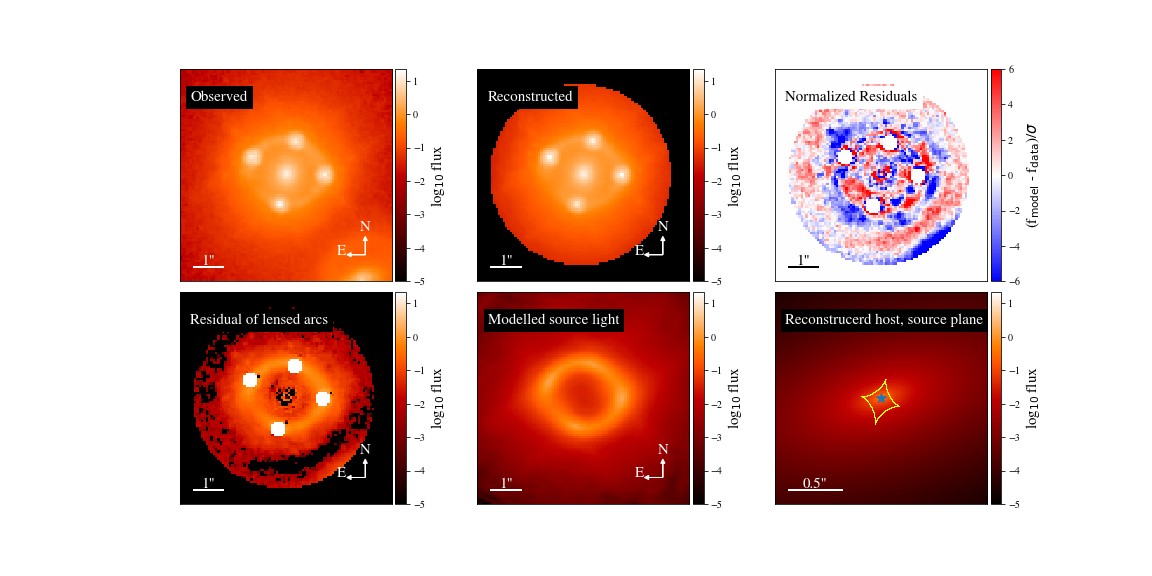
\includegraphics[trim = 40mm 25mm 40mm 25mm, clip, width=0.5\textwidth]{fig/HE0435_inference.png}}&
\subfloat[RXJ1131]{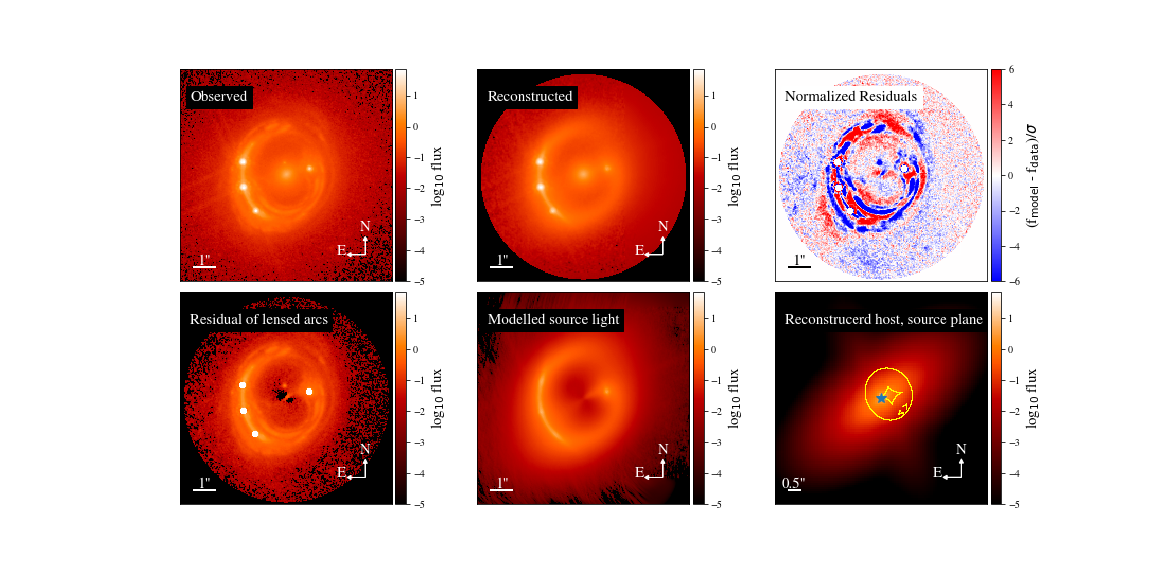
\includegraphics[trim = 40mm 25mm 40mm 25mm, clip, width=0.5\textwidth]{fig/RXJ1131_inference.png}}\\
\subfloat[WFI2033]{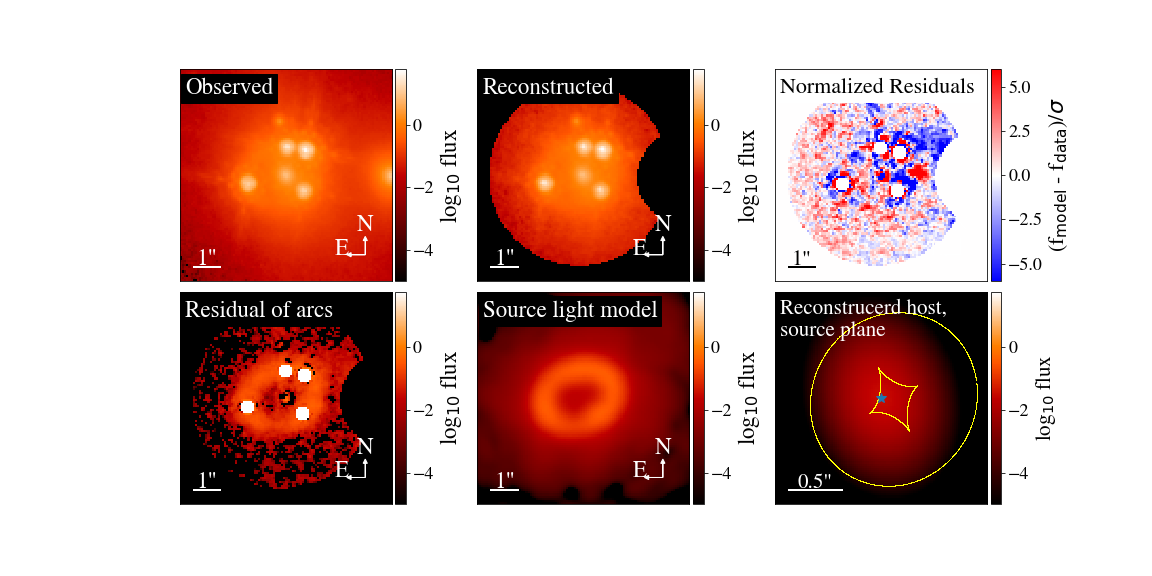
\includegraphics[trim = 40mm 25mm 40mm 25mm, clip, width=0.5\textwidth]{fig/WFI2033_inference.png}}&
\subfloat[SDSS1206]{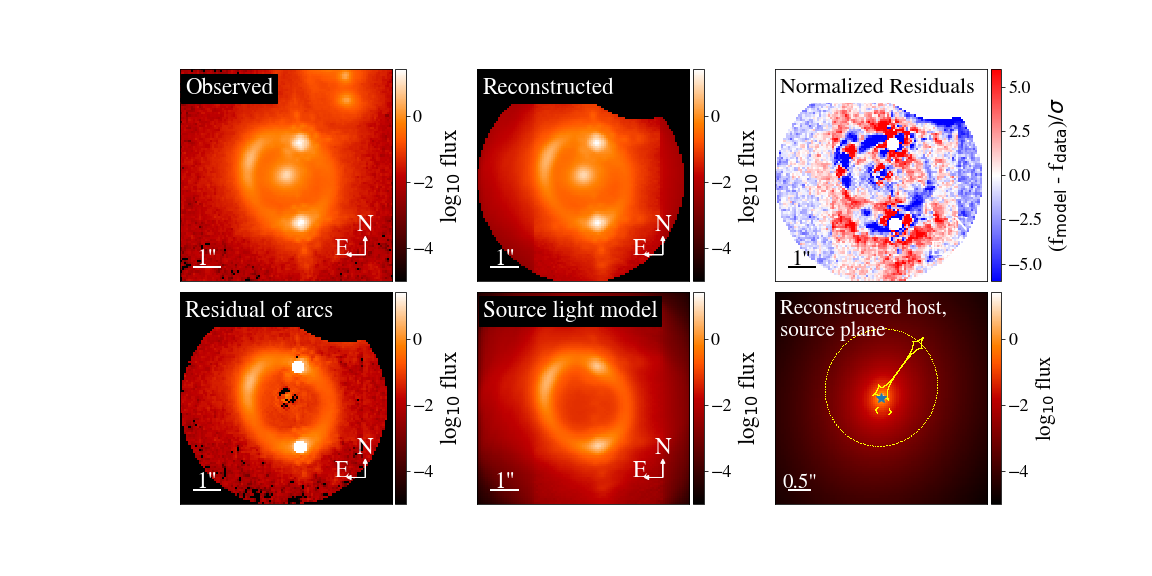
\includegraphics[trim = 40mm 25mm 40mm 25mm, clip, width=0.5\textwidth]{fig/SDSS1206_inference.png}}\\
\subfloat[HE1104]{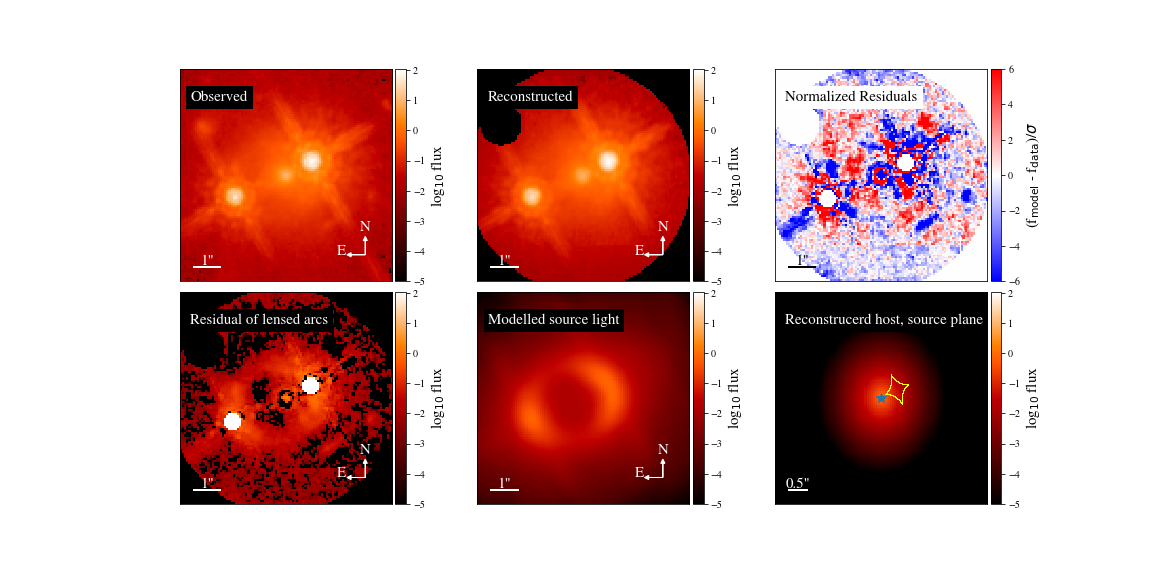
\includegraphics[trim = 40mm 25mm 40mm 25mm, clip, width=0.5\textwidth]{fig/HE1104_inference.png}}&
\subfloat[SDSS0246]{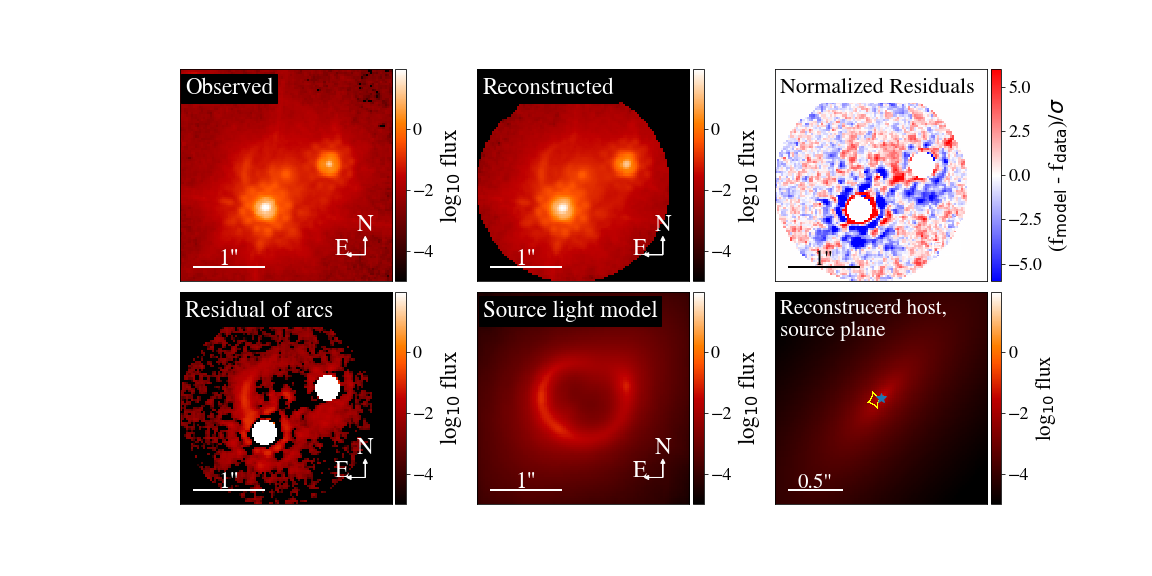
\includegraphics[trim = 40mm 25mm 40mm 25mm, clip, width=0.5\textwidth]{fig/SDSS0246_inference.png}}\\
\subfloat[HS2209]{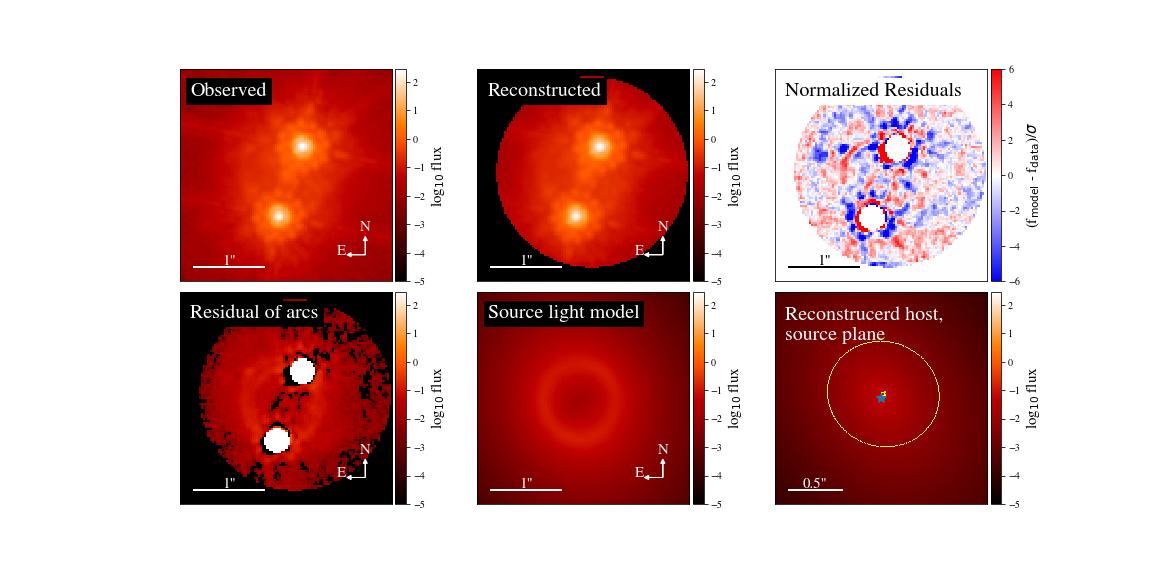
\includegraphics[trim = 40mm 25mm 40mm 25mm, clip, width=0.5\textwidth]{fig/HS2209_inference.png}}&
\subfloat[HE0047]{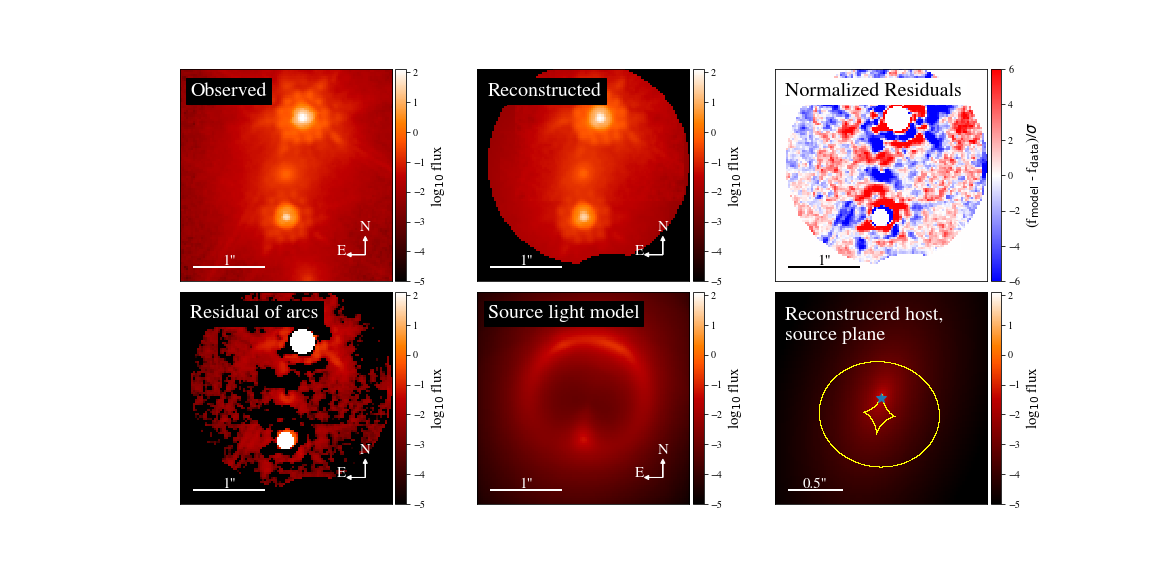
\includegraphics[trim = 40mm 25mm 40mm 25mm, clip, width=0.5\textwidth]{fig/HE0047_inference.png}}\\
\end{tabular}
\caption{\label{fig:image_inference} 
Illustrations of the inference using the best-fit lens model for each system using AGN center noise level boosted approach. For each figure, the panels from left to right are the follows: Top raw: (left to right): (1) observed data, (2) best-fit model (3) residuals divided by the variance; Bottom row: (left to right): (4) data minus the model PSF and deflector  (i.e., pure lensed arc image), (5) the model of the lensed arc, (6) reconstructed host galaxy in the source plane with caustic line drawn as yellow line. Across all the systems, the lensed arc image can be clearly seen by in the fifth panel, indicating a strong evidence of a detection. In panel (3) and (4), we use white regions to indicate the area where the noise level is boosted. 
}
\end{figure*} 

\begin{table*}
\renewcommand{\arraystretch}{1.25}
%\setlength{\tabcolsep}{20pt}
\centering
  \begin{threeparttable}
\caption{Summary of lensed AGN host inference.}\label{tab:host_measure}    
%\resizebox{12cm}{!}{
     \begin{tabular}{cccccccc}
\hline     
(1) & (2) & (3) & (4) & (5) & (6) & (7) & (8) \\    
Object ID & intrinsic Magnitude & Magnitude & Flux Ratio (to Total) & \reff\ & \sersic\ $n$ & stellar population & $\log (M_{*}$)  \\
 & (source plane) & (image plane) & ($\%$) & (arcsec) & & age (Gyr) & (M$_{\odot}$) \\ \hline
HE0435 & $21.49\substack{+0.40\\-0.29}$ & $18.58\substack{+0.30\\-0.23}$ & $36.0\pm11.1$ & $0.28\pm0.02$ & $2.71\pm0.20$ & $1.50$ & $10.91\substack{+0.12\\-0.16}$ \\
RXJ1131$_{\rm bulge}$ & $21.80\substack{+0.23\\-0.19}$ & $18.70\substack{+0.07\\-0.06}$ & $7.1\pm1.4$ & $0.13\pm0.02$ & fix to 4 & $3.00$ & $10.39\substack{+0.08\\-0.09}$ \\
RXJ1131$_{\rm disk}$ & $19.33\substack{+0.17\\-0.15}$ & $17.14\substack{+0.08\\-0.07}$ & $69.2\pm10.1$ & $0.90\pm0.06$ & fix to 1 & $1.50$ & $11.08\substack{+0.06\\-0.07}$ \\
WFI2033 & $21.78\substack{+0.28\\-0.23}$ & $19.07\substack{+0.35\\-0.26}$ & $19.6\pm4.5$ & $0.28\pm0.02$ & $0.52\pm0.01$ & $0.62$ & $10.51\substack{+0.09\\-0.11}$ \\
SDSS1206 & $21.31\substack{+0.23\\-0.19}$ & $18.30\substack{+0.05\\-0.05}$ & $33.3\pm6.4$ & $0.11\pm0.02$ & $4.57\pm0.53$ & $0.62$ & $10.77\substack{+0.08\\-0.09}$ \\
HE1104 & $21.25\substack{+0.16\\-0.14}$ & $19.16\substack{+0.02\\-0.02}$ & $14.0\pm2.0$ & $0.27\pm0.02$ & $1.05\pm0.04$ & $0.63$ & $11.05\substack{+0.06\\-0.07}$ \\
SDSS0246 & $23.44\substack{+0.28\\-0.22}$ & $20.85\substack{+0.08\\-0.07}$ & $4.0\pm0.9$ & $0.44\pm0.08$ & $4.96\pm0.08$ & $0.63$ & $10.75\substack{+0.09\\-0.11}$ \\
HS2209 & $20.72\substack{+0.26\\-0.21}$ & $19.20\substack{+0.04\\-0.04}$ & $12.5\pm2.7$ & $1.96\pm1.28$ & $3.15\pm1.40$ & $1.00$ & $11.04\substack{+0.08\\-0.10}$ \\
HE0047 & $22.92\substack{+0.48\\-0.33}$ & $20.37\substack{+0.20\\-0.17}$ & $2.3\pm0.8$ & $0.32\pm0.15$ & $4.18\pm0.75$ & $0.62$ & $10.91\substack{+0.13\\-0.19}$ \\
\hline
\end{tabular}
%}
\begin{tablenotes}
      \small
      \item Note: $-$ Inference of the host galaxy properties. Column (2)-(6): photometry inference derived using the imaging data in listed Table~\ref{data_set}. Column (7): age of adopted stellar population with stellar metallicity. Column (8): inferred stellar mass. 
\end{tablenotes}    
\end{threeparttable}
\end{table*}


\section{Results}\label{sec:result}
In this section, we describe the approaches and assumptions as used to estimate the stellar populations to our sample. Then, we adopt the population templates to derive their stellar mass of our sample. We study the \mbh-\mstar\ relations and compare our measurements with the ones in the literature to study the evolution.

\subsection{Stellar population and mass}\label{sec:mstar}
%[] Color inference for the first three cases to decide their stellar template. 
Besides the imaging data we analyzed in last section, some of the systems also imaged by the \hst\ through other bands, which could provide the color information. Given that the data observed by other band has less exposure time with lower signal-to-noise (SNR) level, we highlight that we only study the color of the lensed host to determine a decent stellar populations for these systems. Then, these population templates would be applied with the inferred host magnitude (i.e., Table~\ref{tab:host_measure} column (2)) to derive the final stellar mass.

{\bf HE0435} ~ Besides the imaging data by F160W, this system has been observed by the \hst\ through F814W and F555W filters. We adopted the same approach to modelling the data separately at these two band. Considering that the lensed host light in the image plane can be considered as the subtraction of the AGNs and deflectors light which should be less dependent on the lens model, we expect its magnitude in the image plane could be obtained with higher accuracy. Thus, we infer the color of the lensed arcs in the image plane. Based a their magnitudes in three bands, we find a 1.5 Gyr stellar population with solar metallicity could well match this color. More detailed information is presented in Appendix~\ref{app:HE0435}.

{\bf RXJ1131} ~ The host galaxy of RXJ1131 is lensed to a very extended arc in the image plane, which is resolved to the AGNs. The SED fitting of the arc in the image plane can be directly performed using the imaging data. Using the \hst\ imaging data through three filter F814W and F555W and F160W, we adopt the SED fitting result by~\citet{Ding2017b} with the stellar populations of 3 Gyr and 1.5 Gyr (solar metallicity) for its bulge and disk, respectively.

{\bf WFI2033} ~ Besides the F160W filter, four filters including F125W, F140W, F555W, F814W are also available in the \hst\ archive, which has been employed to obtain the color of the host galaxy. Same as the analysis of HE0435, we derive their host magnitudes and infer the host color in the image plane. We find a stellar population with 0.625 Gyr could well match its color (Appendix~\ref{app:WFI2033}).

{\bf HE1104 and the other systems} ~ The imaging data of HE1104 has also been observed by \hst\ through F555W and F814W band. However, given limited exposure time in these two bands, the lensed arcs is too faint to be detected; thus, we couldn't infer the color of the host for HE1104. For the other systems, they do not have the multi-band observation by \hst. For these cases, we adopt the criteria by D20 to assign their stellar populations, i.e., the 1 Gyr and 0.625 Gyr stellar population would be adopted for systems as $z<1.44$ and $z>1.44$, respectively.

A summary of the adopted stellar populations is given in Table~\ref{tab:host_measure}, column~(7). Applying these templates to the filter magnitudes obtained in last section, we derive the stellar mass of our system, Table~\ref{tab:host_measure}, column~(8). Considering the simulating tests by~\citet{Ding2017a} and the fact that we are able to obtain the very consistent host magnitude for the HE0435, RXJ1131 and WFI2033 using the independent approaches, the fidelity of the inferred magnitude are expected to be high. The uncertainty of the \mstar\ estimation are considered as a typical level of $0.2$~dex.

\subsection{The \mbh-\mstar\ relation}\label{sec:relation}
We plot the scaling relation of the \mbh-\mstar\ of our sample, together with the comparison sample as introduced in Section~\ref{sec:sample_select}, in Figures~\ref{fig:scaling_relation}-(a). For the entire sample, we expect that the uncertainty of the \mbh\ (i.e., $0.4~$dex) dominates the error budget. Following D20, we fit the local \mbh-\mstar\ sample as the baseline with a linear relation as:
\begin{eqnarray}
\label{eq:MMlocal}
\log \big( \frac{\mathcal M_{\rm BH}}{10^{7}M_{\odot}})= \alpha + \beta \log(\frac{M_*}{10^{10}M_{\odot}}).
\end {eqnarray}
Comparing with the local sample, we find that our lensed systems appeared to have a slimier offset to the local relations which is consistent to the 32 AGNs by D20 with similar redshift range, indicating a trend of evolution. To study the evolution based on the sample redshift, we parameterize the evolution term as the linear relation by:
\begin{eqnarray}
\label{eq:offset}
\Delta \log \mathcal M_{\rm BH}= \gamma \log (1 + z),
\end{eqnarray} 
where the $\Delta \log \mathcal M_{\rm BH}$ is the offset of the \mbh\ to the local baseline. To make a direct comparison, we first recover the offset plot of Figure~8 in D20. Then we add the data points using our new measurement and show in Figure~\ref{fig:scaling_relation}-(b). We find that the evolution of the offset our sample are well matched to the evolution trend as demonstrated the contrast sample. %Given that we only obtain the measurements from eight lens systems, it is insufficient to fit the offset value quantitively. Nevertheless, 
The apparent consistency in the samples verify the fidelity of our measurement. This result is also support the evolution conclusions drawn by D20.

\begin{figure*}
\centering
\begin{tabular}{c c}
{\includegraphics[height=0.5\textwidth]{fig/MBH-Mstar.pdf}}&
{\includegraphics[height=0.5\textwidth]{fig/MBH-Mstar_vz.pdf}}\\
\end{tabular}
\caption{\label{fig:scaling_relation} 
(left): BH masses vs. stellar mass relations (\mbh-\mstar). The black line and the gray shaded region indicate the best-fit and 1$\sigma$ confidence interval based on the Equation~\ref{eq:MMlocal}.
(right): offset of $\log(\mathcal M_{\rm BH})$ (vs. \mstar) as a function of redshift based on the D20 data using Equation~\ref{eq:offset}. We then plot our new measurement on top of the figure to make direct comparison. 
\todo{HS2209 need to be added. Error bars need to be remarked.}}
\end{figure*} 

\section{Systematic Errors}\label{sec:diss}
We selected to use a set of modelling choices to perform the fitting and the final inference is based on a weighting of top ranked choices. In particular, we treat the two different modelling approaches, i.e., central mask and PSF iteration equally, to derive the averaged results. Of course, with different weighting manner, the combined result would be different. However, as we inspected the results on each choices for each systems, the dispersion of the results by the top ranked choices is usually small and the effect by using different weighting choice is trivial ($<0.1$~dex). In addition, we adopt simple stellar population to derive their stellar mass. 5/8 systems in our sample do not have the color information, and a criteria was adopted to define their stellar population based on their redshift, which would could also introduce the uncertainty in the inferred \mstar.

In any case, we point out that it is the uncertainty of the single-epoch black hole mass estimates (i.e., 0.4~dex) that dominate the error budget in the scaling relations. 

\section{Conclusion}\label{sec:con}
Using eight strongly lensed AGN systems from the H0LiCOW collaboration, we presented the new measurements of the correlations of the supermassive black hole masses and the stellar masses of their host galaxy. We adopt the modern lens modelling techniques to estimate the magnitude host galaxy, defined by the \sersic\ profile. We estimated the \mbh\ of our sample using a set of self-consistent single-epoch estimators to assure the consistency of the correlation.

We directly compare our sample to the recent measurements by~\citet[][D20]{Ding2020a}, who used the similar approaches to derive the \mstar\ and calibrated the \mbh\ using the consistent recipes. The \mbh-\mstar\ of our sample shows the very consistent evolution trend as discovered by D20, as shown in Figure~\ref{fig:scaling_relation}. The consistent result by our sample confirm the evolution of the D20 that the growth of a black hole predates that of its host galaxy.

Our work, once again, confirmed the fidelity of using strong lensing as a tool to study the scaling relation at high redshift. The lensed AGN host galaxy can be accurately recovered using the state-of-the-art lens modelling technique. Even more, with a higher lens magnification effect, the lensed arc by the quadruply imaged sample has demonstrate the higher SNR level (see the Figure~\ref{fig:image_inference}, ``Residual of the lensed arcs'' panel). Apparently, the lensed AGNs have a great potential  to extend to study the \mbh-\mstar\ at even higher redshift range. 

%Finally, we did not consider the selection effect. Besides the mass function, the selection function of the lensed AGNs is also non-trivial. We note that these effects will have to be modelled in the future if the lensed sample is used to infer the evolution. 
The detection of the lensed quasars is going to grow rapidly and sample size of lensed AGNs with the hosts that can be recovered with high fidelity is likely to continue to grow in wide field imaging and spectroscopic surveys~\citep[e.g.,][]{Oguri2010, Agn++15,Mor++16,Sch++16,Ost++17}. The forthcoming launch of the {\it James Webb Space Telescope} and the first light of adaptive optics-assisted extremely large telescopes may provide high-quality imaging data of AGNs at higher redshift (up to $z\sim7$).

\section*{Acknowledgements}
%This work has made use of \lenstronomy~\citep{lenstronomy}, {\sc Astropy}~\citep{Astropy}, {\sc photutils}~\citep{photutils}, {\sc Matplotlib}~\citep{Matplotlib} and standard Python libraries.

This work is based in part on observations made with the NASA/ESA Hubble Space Telescope, obtained at the Space Telescope Science Institute, which is operated by the Association of Universities for Research in Astronomy, Inc., under NASA contract NAS 5-26555. X.D., S.B., and T.T. acknowledge support by the Packard Foundation through a Packard Research fellowship to T.T. \todo{To be updated.}


%%%%%%%%%%%%%%%%%%%%%%%%%%%%%%%%%%%%%%%%%%%%%%%%%%

%%%%%%%%%%%%%%%%%%%% REFERENCES %%%%%%%%%%%%%%%%%%

% The best way to enter references is to use BibTeX:

\bibliographystyle{mnras}
\bibliography{reference} % if your bibtex file is called example.bib


% Alternatively you could enter them by hand, like this:
% This method is tedious and prone to error if you have lots of references
%\begin{thebibliography}{99}
%\bibitem[\protect\citeauthoryear{Author}{2012}]{Author2012}
%Author A.~N., 2013, Journal of Improbable Astronomy, 1, 1
%\bibitem[\protect\citeauthoryear{Others}{2013}]{Others2013}
%Others S., 2012, Journal of Interesting Stuff, 17, 198
%\end{thebibliography}
%%%%%%%%%%%%%%%%%%%%%%%%%%%%%%%%%%%%%%%%%%%%%%%%%%

%%%%%%%%%%%%%%%%% APPENDICES %%%%%%%%%%%%%%%%%%%%%

\appendix

\section{Color inference of the host}
We describe the details of the inference of the stellar population in this section. The template would be then adopted to the photometry by Section~\ref{sec:photometry} to infer the stellar mass.
\subsection{HE0435}\label{app:HE0435}
The HE0435 system are also modelled through ACS/F814W and ACS/F555W (GO-9744; PI: C. S. Kochanek). We derive the magnitude of the lensed galaxy and infer the color of the host in the image plane. To save computer time, we only adopt the {\it PSF iteration} approach and fix the lens mass slope value to 1.9 since it is closer the inference by~\citet[][i.e., $\gamma\sim1.93$]{Wong2017}. We illustrate the lens model for the other two band in Figure~\ref{fig:app_HE0435}-(a), (b). The accuracy of the inferred host magnitude in the image plane is considered to be robust, and we consider them to have the same uncertainty as the F160W band inference. Having obtained the magnitude of the lensed host at three band, we use {\sc gsf} package to select the best stellar population from a range of [0.625, 0.8, 1.0, 1.5, 2.0, 3.0] Gyr with solar metallicity. Finally, a stellar population with age of 1.5 Gyr demonstrated the best matching to the color, which is selected to the final inference, see Figure~\ref{fig:app_HE0435}-(c).


\begin{figure*}
\centering
\subfloat[HE0435 F555W]{\includegraphics[ width=0.8\textwidth]{fig/HE0435_f555w_inference.pdf}}\\
\subfloat[HE0435 F814W]{\includegraphics[ width=0.8\textwidth]{fig/HE0435_f814w_inference.pdf}}\\
\subfloat[Host galaxy stellar template inference]{\includegraphics[ width=0.5\textwidth]{fig/HE0435_host_color.pdf}}\\
\caption{\label{fig:app_HE0435} 
Illustrations of the inference of HE0435 using the data at the other two bands. Top two panels: best-fit model of the lensed arcs shown as Figure~\ref{fig:image_inference}. Bottom panel: SED inference of the color using the three band inference.}
\end{figure*} 

%\subsection{RXJ1131}\label{app:RXJ1131}
%Using the three band data including  ACS/F814W and ACS/F555W and NIC2/F160W (GO-9744; PI: C. S. Kochanek), we preform the SED fitting in the imaging plane directly pixel by pixel in Figure~\ref{fig:app_RXJ1131}. \ding{This part is actually done by Takahiro in~\citep{Ding2017b}. The image of the fitted age looks noisy, but it is in the range of the [9.25 - 9.50] (logAge), i.e. [1.5, 3.0] (Gyr). We can remove this A2 but only mention the fitting is done 2017 in that paper.}
%\begin{figure}
%\centering
%{\includegraphics[width=0.25\textwidth]{fig/map_age_zRXJ_1131.pdf}}\\
%\caption{\label{fig:app_RXJ1131} 
%Illustrations of the SED fitting of the galaxy age pixel by pixel.  }
%\end{figure} 

\subsection{WFI2033}\label{app:WFI2033}
WFI2033 is also observed by other four band data including WFC3/F125W (GO-12874; PI: D. Floyd), WFC3/F140W (GO-13732; PI: A. Nierenberg), ACS/F555W+F814W  (GO-9744; PI: C. S. Kochanek). Similar to Section~\ref{app:HE0435}, the inference of the lensed arcs of WFI2033 have been fitted through five band. The lensed models are presented in the Figure~\ref{fig:app_WFI2033}-(a)$-$(d). Note that, limited by its exposure time, the data quality by F125W is not ideal and the host information could not be well extracted. Thus, we does not take the inference by F125W into account in the color inference. Finally, we find the stellar population with 0.625 Gyr age could well matched the color, i.e., Figure~\ref{fig:app_WFI2033}-(e).
\begin{figure*}
\centering
\subfloat[WFI2033 F125W \todo{remove arrows}]{\includegraphics[ width=0.8\textwidth]{fig/WFI2033_f125w_inference.pdf}}\\
\subfloat[WFI2033 F140W \todo{remove arrows}]{\includegraphics[ width=0.8\textwidth]{fig/WFI2033_f140w_inference.pdf}}\\
\subfloat[WFI2033 F555W]{\includegraphics[ width=0.8\textwidth]{fig/WFI2033_f555w_inference.pdf}}\\
\subfloat[WFI2033 F814W]{\includegraphics[ width=0.8\textwidth]{fig/WFI2033_f814w_inference.pdf}}\\
\subfloat[Host galaxy stellar template inference]{\includegraphics[ width=0.5\textwidth]{fig/WFI2033_host_color.pdf}}
\caption{\label{fig:app_WFI2033} 
Same as Figure~\ref{fig:app_WFI2033} but for WFI2033. The inference of the lensed arcs is not clear in the F125W data, and thus the SED fitting is done through the other four bands.}
\end{figure*} 
%%%%%%%%%%%%%%%%%%%%%%%%%%%%%%%%%%%%%%%%%%%%%%%%%%


% Don't change these lines
\bsp	% typesetting comment
\label{lastpage}
\end{document}

% End of mnras_template.tex